\documentclass[10pt,a4paper]{article}
\usepackage[margin=22mm]{geometry}
\usepackage[T1]{fontenc}
\usepackage{lmodern,graphicx,amsmath,booktabs,array,microtype}
\usepackage[hidelinks]{hyperref}
\usepackage{caption}
\captionsetup{font=small,labelfont=bf}
\graphicspath{{../../artifacts/oversight_simulation/figures/}}
\newcommand{\QueueCorrect}{5.45}
\newcommand{\QueueWrong}{1.06}
\newcommand{\QueueUnfinished}{5.49}
\newcommand{\GroupCorrect}{5.29}
\newcommand{\GroupWrong}{1.04}
\newcommand{\GroupUnfinished}{5.67}
\newcommand{\AwareCorrect}{5.41}
\newcommand{\AwareWrong}{1.06}
\newcommand{\AwareUnfinished}{5.53}
\newcommand{\StickyCorrect}{5.61}
\newcommand{\StickyWrong}{1.03}
\newcommand{\StickyUnfinished}{5.35}
\newcommand{\ManualCorrect}{5.18}
\newcommand{\ManualWrong}{0.79}
\newcommand{\ManualUnfinished}{6.03}
\newcommand{\PrimaryDelta}{-0.156}
\newcommand{\PrimaryLow}{-0.270}
\newcommand{\PrimaryHigh}{-0.043}
\newcommand{\ControlDelta}{-0.115}
\newcommand{\ControlLow}{-0.170}
\newcommand{\ControlHigh}{-0.059}
\newcommand{\ShortDelta}{+0.198}
\newcommand{\ShortLow}{+0.081}
\newcommand{\ShortHigh}{+0.315}
\newcommand{\LargeDelta}{+0.865}
\newcommand{\LargeLow}{+0.727}
\newcommand{\LargeHigh}{+1.002}

\setlength{\parskip}{4pt}
\setlength{\parindent}{0pt}
\title{Source-Aware Review of Concurrent Agent Outputs:\\A Computational Study of Familiarity, Capacity and Error}
\author{OverseeingManyLLMs research project\\\small Separate computational draft; no participant observations}
\date{13 September 2026}
\begin{document}
\maketitle
\begin{abstract}
Concurrent language-model task workers can produce more material than a reviewer
can inspect. Arranging questions around their shared source may reduce repeated
orientation, but the same saving may be available through ordinary source-aware
queue navigation. We study this distinction with a discrete-event simulation
using 36 original TAT-QA questions, six real financial-report contexts and genuine
saved model drafts. Reviewer behavior and arrivals are explicitly modeled rather
than observed. A committed sensitivity design contains 66 settings and 31,680
paired runs. Grouping improves mean correct releases over arrival-order review in
24 settings, ties in two and reduces them in 40. It never exceeds a queue with the
same bounded source-aware navigation and no grouping overhead. Costly orientation
and short familiarity can favor reordering, whereas persistent familiarity,
carryover errors and cheap manual construction weaken or reverse apparent
benefits. The contribution is a reproducible conditional operating map and an
information-equivalent control. It provides no evidence of measured human
efficiency or workload improvement.
\end{abstract}

\section{Question and evidence boundary}
A review desk can preserve a source, an answer and its approval controls while
other agent requests arrive. It can also group related questions. The research
question is whether grouping improves useful completion within a fixed review
budget, and which mechanism would explain that improvement. Showing several
questions together need not be beneficial if a conventional queue can already
visit them consecutively. Conversely, grouping could affect comprehension or
navigation choices in ways a timing simulation cannot establish.

We therefore compare explicit navigation strategies under a common source-memory
model. We neither grant grouping a speed multiplier nor withhold source reuse
from a queue. Separate outcomes count correct releases, incorrect releases and
unfinished work. More releases alone are not better oversight. A manual condition
also tests the assumption that reviewing these particular drafts is useful.

The inputs come from the existing matched review study, whose prospective human
protocol and position paper remain unchanged. TAT-QA combines financial tables
and accompanying text with human-written questions and annotations\cite{tatqa}.
We retain all 36 selected questions and actual replica-0 Qwen2.5-7B-Instruct drafts,
including errors and missing answers. Only 7/36 drafts are jointly correct in
answer and scale; five displayed fields are empty or unsupported. These values
describe saved model outputs, not reviewer competence.

\begin{center}
\small
\begin{tabular}{p{.27\linewidth}p{.66\linewidth}}
\toprule
Evidence layer & Status in this study\\\midrule
Financial tables and text & Real report material represented by the benchmark\\
Questions and references & Original benchmark questions and annotation labels\\
Initial drafts & Actual saved generations; no new inference or artificial errors\\
Workers, arrivals and cutoff & Constructed supervision application\\
Review timing and outcomes & Simulated under analyst-selected assumptions\\
Human behavior & Unmeasured; no participants, ratings or practice records used\\\bottomrule
\end{tabular}
\end{center}

\clearpage
\section{Shared reviewer and event protocol}
A question is one user-valued goal. All requests remain accounted for from offer
through release or cutoff. Receipt during a review cannot replace the active
artifact. Approval and release are distinct actions bound to an exact output
version. A correction creates a new version. Deferral retains the original output;
rejection and approval without release remain unfinished. The simulator calls the
existing review engine's transition and invariant functions. It does not implement
a looser simulation-only release rule.

Review time is the sum of orientation, question interpretation, verification or
construction, decision interaction and release interaction. A grouped session
adds its declared overhead. For source $s$, orientation is $S f_s$ on a first
visit. On return it is
\begin{equation}
 O_s=S f_s\left[r+(1-r)\left(1-e^{-g_s/\tau-k_s/\kappa}\right)\right],
\end{equation}
where $g_s$ is elapsed simulated time since the last completed review decision on
that source, $k_s$ counts intervening decisions, and $r=0.1$. The public source-size
factor $f_s$ is character count divided by 3,200, clipped to $[.75,1.25]$.
All six selected sources have $f_s=.75$, so their first-visit orientation is
$.75S$; the size factor does not discriminate difficulty in these matched packets.
There is no additional switching charge. Consecutive FIFO questions receive the
same familiarity saving as grouped questions. A completed failed construction
can also refresh source familiarity.

Question, verification and construction times use a common wording factor
$1+\min(40,\text{word count})/80$ and mean-one lognormal jitter with $\sigma=.2$.
Neither the timing rule nor the navigation policy receives gold derivations or
future outcomes. Random draws are keyed by seed, question, attempt and component,
so matched methods share potential outcomes wherever their paths permit.

\begin{center}\small
\begin{tabular}{p{.40\linewidth}p{.52\linewidth}}
\toprule
Assumed component & Reference and declared sensitivities\\\midrule
Orientation coefficient $S$ & 25 s; also 0, 5, 75 s\\
Memory $\tau,\kappa$ & 600 s, 8 decisions; also 45 s, 2; effectively persistent\\
Question / verification & 8 / 18 s; verification also 8, 40 s\\
Detected-error construction & 45 s\\
Manual or empty-draft construction & 45 s; also 20, 90 s\\
Decision / release interaction & 2 / 2 s\\
Grouped-session overhead & 4 s; also 0, 12 s\\
Deferral & Eligible again after 45 s, at most two attempts\\\bottomrule
\end{tabular}\end{center}

\subsection{Fallible outcomes and limited authority}
The simulated environment uses annotations to determine whether the initial
draft is correct. A wrong nonempty draft is detected with probability $d$ and
successfully corrected with probability $c$ after detection. Undetected errors are
approved incorrectly. A correct draft can be damaged with probability $h$.
Manual and empty-draft constructions succeed with probability $m$. Successful
simulated constructions copy only that question's annotated answer and scale.
An unsuccessful construction uses an explicit simulation sentinel, not a generated
financial assertion. Half of failed constructions recognize inability and defer,
then reject on a second recognized failure. Other failures release a wrong answer.

The ideal setting is $(d,c,h,m)=(1,1,0,1)$. Higher and limited effectiveness use
$(.85,.85,.02,.75)$ and $(.55,.60,.08,.50)$. A separate stress hazard of
0, .08 or .20 can spoil an otherwise correct answer after another question from
the same source. It applies equally to all methods. These are assumptions, not
inferences from model accuracy or fitted measurements of financial reviewers.
Source grouping never grants shared approval authority.

\clearpage
\section{Comparisons, design and numerical uncertainty}
\begin{center}\small
\begin{tabular}{p{.22\linewidth}p{.69\linewidth}}
\toprule
Policy & Public next-request rule\\\midrule
FIFO Q & Earliest received eligible request, then stable question identifier\\
Grouped G & FIFO starts up to three available questions from one source; finish
that set, then return to FIFO. Charge overhead for a multi-question group.\\
Source-aware Q & G's identical bounded selection, without grouping cards or overhead\\
Sticky Q & Continue on the last source while eligible related questions remain\\
Manual M & FIFO selection and source-only construction, with no draft\\\bottomrule
\end{tabular}\end{center}
All selectors see arrived identifiers, actual source identity, receipt times and
pending status. They cannot see correctness, future arrivals or random outcomes.
No policy waits to assemble a group. G assumes use of grouping whenever possible;
it does not model observed uptake. FIFO describes a strategy, not a constraint of
the real queue interface, where a person can already select related questions.

The original scenario offers twelve questions for 540 seconds. Arrivals reproduce
the matched schedule, at $0,4,\ldots,20$ and $180,184,\ldots,200$ seconds plus .25 s
delivery. Each of three packets has two sources with six questions each.
Separate stress scenarios use 6, 12, 24 or 36 distinct questions, 270, 540 or 900 s
capacity, burst/two-wave/spread arrivals and interleaved/source-blocked order.
Smaller loads use declared public prefixes; larger ones union packets without
duplicating goals. Costs, effectiveness, memory and carryover are varied in
prespecified compact subsets, not a fitted distribution of real workloads.

The frozen design comprises 66 settings, three rotations, 32 seeds and five
policies, totaling 31,680 runs. A preliminary 64-seed forecast was reduced before
comparative outcomes; all parameter settings were retained. The sources were
previously inspected and do not establish six independent reports. Rotations,
questions and seeds are not people or new organizations.

For each setting, paired rotation differences are averaged within seed. Intervals
are the mean plus or minus $1.96$ Monte Carlo standard errors across 32 seed
blocks. They quantify numerical integration uncertainty conditional on the fixed
model and sources. More seeds cannot validate a memory function or reduce
uncertainty about an unmeasured reviewer population. We report each setting
separately and do not pool the sensitivity grid into a global effectiveness claim.

\section{The original setting favors simpler controls}
At $S=25$ s (18.75 s on first visit), long memory and higher effectiveness, G minus Q is
\PrimaryDelta{} correct releases per twelve offered, with Monte Carlo interval
[\PrimaryLow, \PrimaryHigh]. G minus source-aware Q is \ControlDelta{}
[\ControlLow, \ControlHigh]. Seed-block G--Q wins/ties/losses are 3/16/13.

\begin{center}\small
\begin{tabular}{lrrr}
\toprule Policy & Correct releases & Incorrect releases & Unfinished\\\midrule
FIFO Q & \QueueCorrect & \QueueWrong & \QueueUnfinished\\
Grouped G & \GroupCorrect & \GroupWrong & \GroupUnfinished\\
Source-aware Q & \AwareCorrect & \AwareWrong & \AwareUnfinished\\
Sticky Q & \StickyCorrect & \StickyWrong & \StickyUnfinished\\
Manual M & \ManualCorrect & \ManualWrong & \ManualUnfinished\\\bottomrule
\end{tabular}\end{center}
Every offered question remains in this table. An answer must be jointly correct
in content and scale, approved and released at its current version. Construction
failures, never-selected requests, rejections and cutoff work are retained. The
manual comparison is small and numerically uncertain here: Q--M is $+.271$
$[-.007,.548]$ and G--M is $+.115$ $[-.152,.381]$ correct releases. These intervals
are not evidence of human equivalence or of preserved quality. Q--M holds
FIFO navigation fixed. G--M additionally changes ordering, so it compares whole
workflows rather than isolating draft availability.

\clearpage
\section{Conditional operating regions}
\begin{figure}[h!]
\centering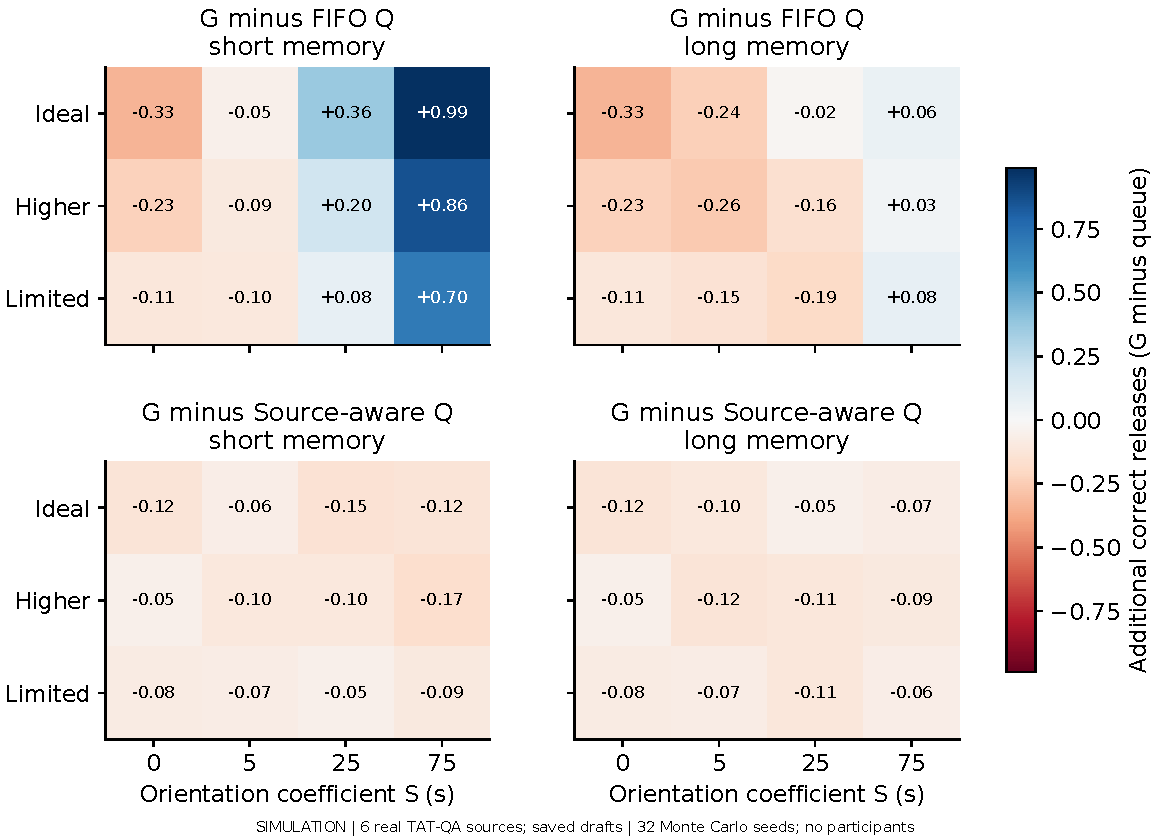
\includegraphics[width=.94\linewidth]{orientation_effectiveness.pdf}
\caption{Simulated additional correct releases for G under the original workload.
Real TAT-QA sources and actual drafts are fixed inputs; every timing and reviewer
parameter is assumed. Blue favors G and red favors the indicated queue. Both
rows use the same centered scale. Means average three packets and 32 Monte Carlo
seeds, not human participants.}
\end{figure}
With $S=25$ s, shortening memory changes G--Q from \PrimaryDelta{}
to \ShortDelta{} [\ShortLow, \ShortHigh]. At $S=75$ s with short memory it is
\LargeDelta{} [\LargeLow, \LargeHigh]. That gain also increases wrong releases
from .688 to .833. More correct releases can therefore accompany greater risk.
Ideal-reviewer cells expose the capacity effect without error uncertainty, while
fallible cells show whether it persists under the assumed detection and repair rates.

Across the declared grid G has positive, tied and negative mean differences
against FIFO in 24, 2 and 40 settings. Against bounded source-aware Q the counts
are 0, 4 and 62. Three ties are the zero-overhead cases, where equality follows
mechanically from shared selection and random inputs. The fourth has six questions
and a fifteen-minute budget. All assisted policies then average 5.031 correct,
.938 incorrect and .031 unfinished. This is ample capacity with shared fallibility,
not proof of equivalent human interfaces.

\clearpage
\begin{figure}[h!]
\centering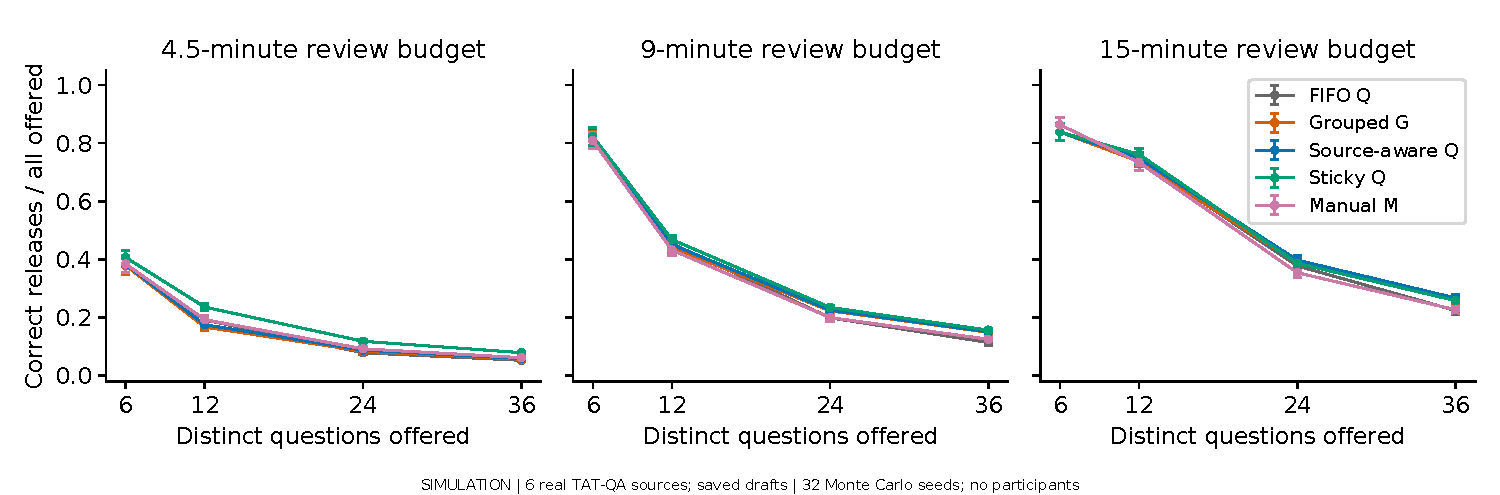
\includegraphics[width=\linewidth]{demand.pdf}
\caption{Simulated correct releases divided by all distinct offered questions.
Arrivals, capacity and reviewer behavior are constructed. Error bars are conditional
Monte Carlo intervals across 32 seeds, with three source-packet rotations per seed.
No point represents a participant. Lines connect the declared load settings.}
\end{figure}
Higher demand creates more opportunity for ordering to change the completed set.
At 36 questions and fifteen minutes, G--Q is $+1.333$ $[1.068,1.599]$ answers,
but G still trails source-aware Q by .208. With 24 questions in two waves,
interleaving yields $+.583$ $[.462,.704]$ for G--Q, whereas source-blocked ordering
yields $-.042$ $[-.090,.007]$. A FIFO queue already adjacent by source leaves
little repeated orientation to save.

\begin{figure}[h!]
\centering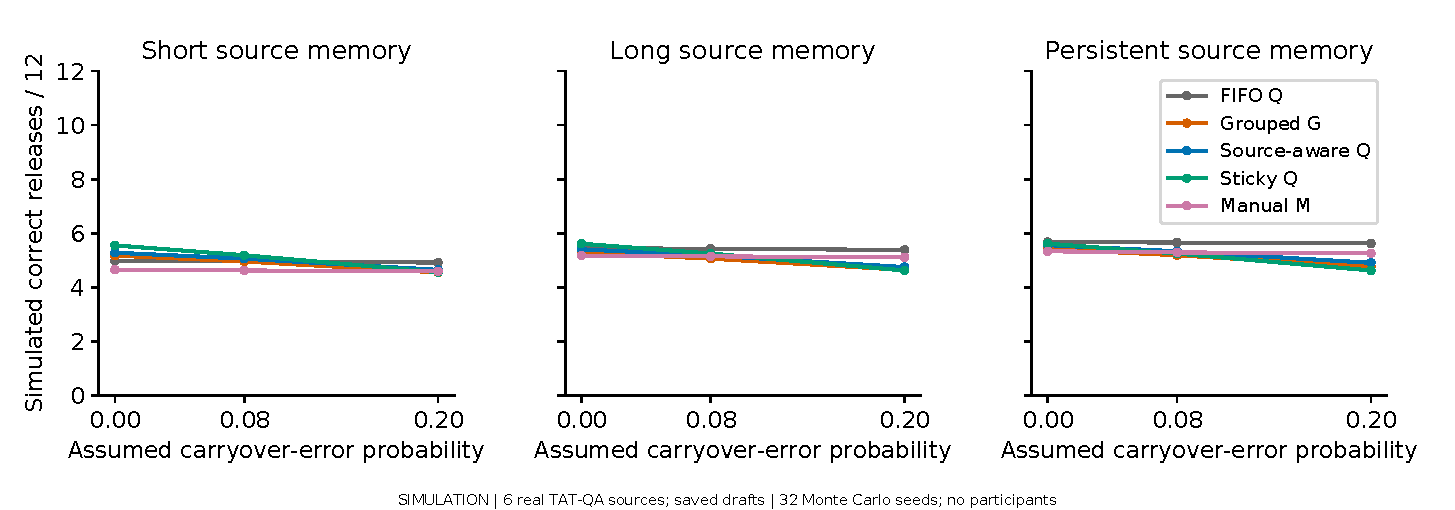
\includegraphics[width=\linewidth]{memory_carryover.pdf}
\caption{Simulated correct releases under different memory and same-source
carryover assumptions. The hazard applies to every method, not just grouping.
Real source material does not validate these behavioral probabilities.}
\end{figure}
Carryover challenges the same mechanism that makes consecutive-source work
efficient. With long memory and hazard .20, G--Q becomes $-.740$
$[-.925,-.555]$. Wrong releases rise from 1.042 to 1.688 for G, compared with
1.062 to 1.125 for FIFO. Sticky-source review can also lose its advantage. This is
a model-based exposure effect, not evidence that financial reviewers actually
make these carryover errors.

\subsection{A conditional break-even explanation}
For the same attempted work and success path, saved review time is orientation
saved minus grouping overhead. That balance matters only if it permits another
full decision and release before cutoff. Summing orientation over different
completed subsets is not a valid causal explanation by itself. Delayed unrelated
work and harmful carryover also matter. At zero overhead, G and source-aware Q are
identical by induction over event times. With positive overhead, changing eligible
sets can change paths, so we assert no general dominance theorem. The finite-grid
result supports navigation as the simpler explanation, without proving that real
cards have no comprehension benefit.

\clearpage
\begin{figure}[h!]
\centering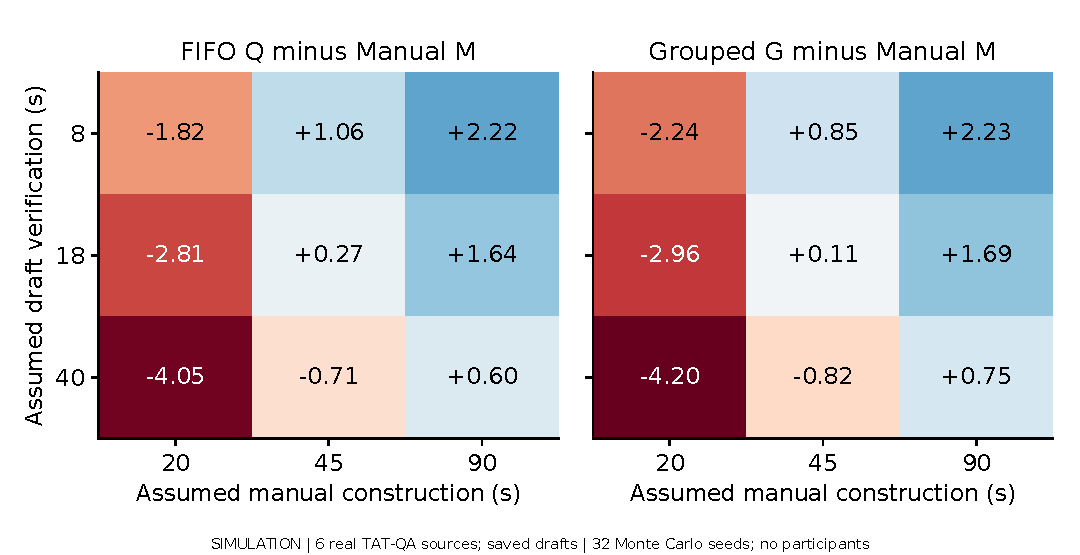
\includegraphics[width=.83\linewidth]{draft_assistance.pdf}
\caption{Simulated assistance effect in correct releases relative to manual work.
Positive values favor drafts; negative values favor manual construction. Inputs
are genuine imperfect drafts, while verification, construction and reviewer
effectiveness are analyst assumptions. Both panels use one symmetric color scale.}
\end{figure}
\section{Interpretation, limitations and next evidence}
When manual construction is cheap and checking is expensive, source-only work
outperforms reviewing these drafts. G--M is $-4.198$ $[-4.528,-3.868]$ at
20-second manual construction and 40-second verification. At 90-second manual
construction and 8-second verification it is $+2.229$ $[2.040,2.418]$. Those
declared extremes identify a boundary, not a human assistance effect.

The central contribution is a controlled conditional comparison that separates
source-aware navigation from grouping overhead while retaining real questions,
wrong drafts, unfinished work and exact-version releases. Queues, batching and
memory models are established mechanisms. Interruption research distinguishes
returning to a task from recovering context\cite{iqbal}; scheduling research
already studies setup/batching tradeoffs\cite{potts}. Neither source calibrates
this financial-review model. Our function, numerical ranges, feature-use rule and
question-independent random errors remain unvalidated. Shared errors, skill
differences, evidence understanding and adoption choices could alter the outcomes.

All 31,680 command streams replayed, 200,286 released answers were independently
re-scored, and 120 traces matched the ordinary atomic review engine. Twelve focused
tests check information, timing and authority boundaries. The 52 protected human
study and manuscript files are unchanged. These checks establish software
accounting, not reviewer comprehension. The CPU batch took 265 seconds with no
new inference. Saved commands, inputs, configurations, figures and reproduction
instructions accompany this separate draft.

The next observations should measure orientation after consecutive and intervening
questions, actual grouping interaction, source-aware queue navigation, detection
and repair, manual construction and unit carryover. They can calibrate or falsify
the modeled operating regions. The preserved prospective study remains useful;
any added automatic source-aware comparator needs a separately declared design.
This computational study supports a systems-and-simulation finding, while human
correctness, efficiency, control and workload benefits remain unmeasured.

\begin{thebibliography}{9}\small
\bibitem{tatqa} F. Zhu et al. 2021. TAT-QA: A Question Answering Benchmark on a
Hybrid of Tabular and Textual Content in Finance. ACL-IJCNLP, 3277--3287.
\url{https://aclanthology.org/2021.acl-long.254/}.
\bibitem{iqbal} S. T. Iqbal and E. Horvitz. 2007. Disruption and Recovery of
Computing Tasks: Field Study, Analysis, and Directions. CHI, 677--686.
\url{https://www.erichorvitz.com/CHI_2007_Iqbal_Horvitz.pdf}.
\bibitem{potts} C. N. Potts and M. Y. Kovalyov. 2000. Scheduling with batching:
A review. European Journal of Operational Research 120(2), 228--249.
\url{https://doi.org/10.1016/S0377-2217(99)00153-8}.
\end{thebibliography}
\end{document}
